%
%===============>>  Сторожук Модуль 5 <<=============
%
\setmodule{5}

%BEGIN_FOLD % ====>>_____ Занятие 1 _____<<====
\begin{class}[number=1]
	
	\begin{listofex}
		\item   Занятие 1
	\end{listofex}
\end{class}
%END_FOLD

%BEGIN_FOLD % ====>>_____ Занятие 2 _____<<====
\begin{class}[number=2]
	\begin{listofex}
		\item Занятие 2
	\end{listofex}
\end{class}
%END_FOLD

%BEGIN_FOLD % ====>>_ Домашняя работа 1 _<<====
\begin{homework}[number=1]
	\begin{listofex}
		\item  Найти значения выражения:
		\begin{tasks}(2)
			\task \( 2^{\log_26-3} \)
			\task \( 7\cdot5^{\log_54} \)
			\task \( 6^{5\log_63} \)
			\task \( \log_2112-\log_27 \)
			\task \( \log_340,5+\log_36 \)
			\task \( 6^{3\log_62} \)
			\task \( \dfrac{\log_318}{2+\log_32} \)
			\task \( (\log_381)\cdot(\log_6216) \)
		\end{tasks}
		\item 	
			\begin{minipage}[t]{\bodywidth}
			На рисунке изображён график функции \[ f(x)=kx+b. \] Найдите \(f(-200)\).
		\end{minipage}
		\hspace{0.02\linewidth}
		\begin{minipage}[t]{\picwidth}
			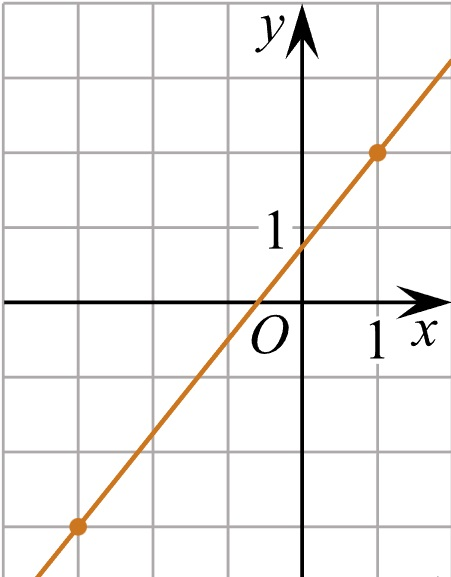
\includegraphics[align=t, width=\linewidth]{../../pics/G101M4C4-1}
		\end{minipage}
		\item 
		\begin{minipage}[t]{\bodywidth}
			На рисунке изображены графики функций \( f(x)=4x^2-25x+41 \) и \( g(x)=ax^2+bx+c \), которые пересекаются в точках \(A\) и \(B\). Найдите абсциссу  \( B \).
		\end{minipage}
		\begin{minipage}[t]{\picwidth}
			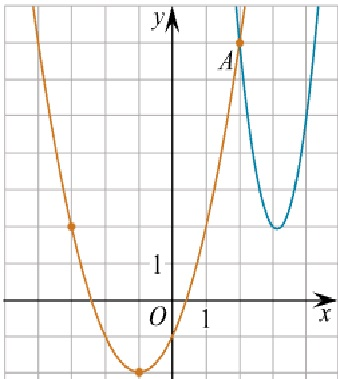
\includegraphics[align=t, width=\linewidth]{../../pics/G111M3PP-1}
		\end{minipage}
	\end{listofex}
\end{homework}
%END_FOLD

%BEGIN_FOLD % ====>>_____ Занятие 3 _____<<====
\begin{class}[number=3]
	\begin{listofex}
		\item Занятие 3
	\end{listofex}
\end{class}
%END_FOLD

%BEGIN_FOLD % ====>>_____ Занятие 4 _____<<====
\begin{class}[number=4]
	\begin{listofex}
		\item Занятие 4
	\end{listofex}
\end{class}
%END_FOLD

%BEGIN_FOLD % ====>>_ Домашняя работа 2 _<<====
\begin{homework}[number=2]
	\begin{listofex}
		\item ДЗ 2
	\end{listofex}
\end{homework}
%END_FOLD

%BEGIN_FOLD % ====>>_____ Занятие 5 _____<<====
\begin{class}[number=5]
	\begin{listofex}
		\item Занятие 5
	\end{listofex}
\end{class}
%END_FOLD

%BEGIN_FOLD % ====>>_____ Занятие 6 _____<<====
\begin{class}[number=6]
	\begin{listofex}
		\item Занятие 6
	\end{listofex}
\end{class}
%END_FOLD

%BEGIN_FOLD % ====>>_ Домашняя работа 3 _<<====
\begin{homework}[number=3]
	\begin{listofex}
		\item ДЗ 3
	\end{listofex}
\end{homework}
%END_FOLD

%BEGIN_FOLD % ====>>_____ Занятие 7 _____<<====
\begin{class}[number=7]
	\begin{listofex}
		\item Занятие 7
	\end{listofex}
\end{class}
%END_FOLD

%BEGIN_FOLD % ====>>_ Проверочная работа _<<====
\begin{exam}
	\begin{listofex}
		\item Проверочная работа
	\end{listofex}
\end{exam}
%END_FOLD